\begin{mdframed}[style=warning]
	\textbf{Conceptos}
		\begin{enumerate}
			\item Un globo de aire caliente se llena con aire calentado por un quemador en la base. ¿Por qué debe calentarse el aire? ¿Cómo se controla el ascenso y el descenso?
			\item Si la corriente de aire de una secadora de cabello se dirige hacia una pelota de ping pong, la pelota puede levitar. ¿Por qué?
			\item ¿Por qué los pilotos de avión prefieren despegar con el avión contra el viento?
		\end{enumerate}
\end{mdframed}






\begin{mdframed}[style=warning]
	\begin{ejercicio}
		La figura muestra una bola de hierro suspendida por un hilo de masa despresiable de un cilindro vertical que flota parcialmente sumergido en agua. El cilindro tiene una altura de $6cm$, un área frontal de $12cm^2$ en la parte superior e inferior y una densidad de $0.3g/cm^3$, y $2cm$ de su altura están por encima de la superficie del agua. ¿Cuál es el radio de la bola de hierro?
		
		\begin{figure}[H]
			\centering
			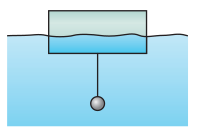
\includegraphics[scale=0.5]{./img/p1.png}
		\end{figure}
	\end{ejercicio}
\end{mdframed}


























\begin{mdframed}[style=warning]
	\begin{ejercicio}
		Un bloque cúbico con densidad $\rho _B$ y lados de longitud $L$ flota en un líquido con densidad mayor a $\rho _L$. $a)$ ¿Qué fracción del volumen del bloque está sobre la superficie del líquido? $b)$ El líquido es más denso que el agua ($\rho _A$) y no se mezcla con ella. Si se vierte agua en la superficie del líquido, ¿qué espesor debe tener la capa del agua para que su superficie esté al ras de la cara superior del bloque? $c)$ Calcule la profundidad de la capa de agua en el inciso $b)$ si el líquido es mercurio, el bloque está hecho de hierro y la longitud de su lado es de $10cm$.
	\end{ejercicio}
\end{mdframed}















%%%